\documentclass[12pt, twoside]{article}
\usepackage[letterpaper, margin=1in, headsep=0.5in]{geometry}
\usepackage[english]{babel}
\usepackage[utf8]{inputenc}
\usepackage{amsmath}
\usepackage{amsfonts}
\usepackage{amssymb}
\usepackage{tikz}
\usepackage{yhmath}
%\usetikzlibrary{quotes, angles}

\usepackage{graphicx}
\usepackage{enumitem}
\usepackage{multicol}

\usepackage{fancyhdr}
\pagestyle{fancy}
\fancyhf{}
\renewcommand{\headrulewidth}{0pt} % disable the underline of the header

\fancyhead[RE]{\thepage}
\fancyhead[RO]{\thepage \\ Name: \hspace{3cm}}
\fancyhead[L]{BECA / Dr. Huson / 10th Grade Geometry\\* 12 February 2020}

\begin{document}
\subsubsection*{8.11 Do Now: Compound areas}
 \begin{enumerate}
  \item Find the area of the shape shown below composed of a rectangle and two triangles.
    \begin{flushright}
    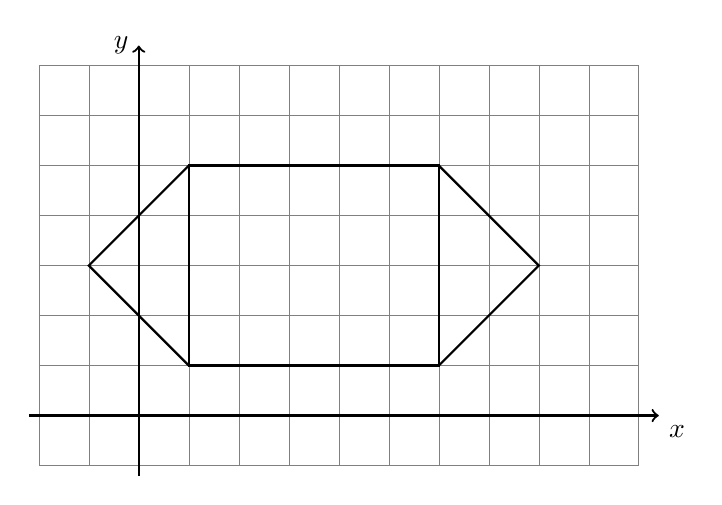
\begin{tikzpicture}[scale=.635]
      \draw [help lines] (-2,-1) grid (10,7);
      \draw [thick, ->] (-2.2,0) -- (10.4,0) node [below right] {$x$};
      \draw [thick, ->] (0,-1.2)--(0,7.4) node [left] {$y$};
      \draw [thick] (1,1)--(6,1)--(6,5)--(1,5)--cycle;
      \draw [thick] (6,1)--(8,3)--(6,5);
      \draw [thick] (1,1)--(-1,3)--(1,5);
      %\draw [thick] (6,1) arc (-90:90:2);
    \end{tikzpicture}
  \end{flushright} \vspace{1cm}
  
  \item The figure shows a rectangle 3 cm wide and 2 cm high.
  \begin{center}
    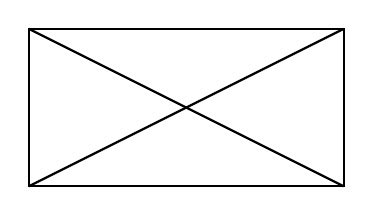
\begin{tikzpicture}%[scale=0.9]
      \coordinate (A) at (0, 0); %[label=above left:$P$]
      \coordinate (B) at (4, 0);
      \coordinate (C) at (4, 2);
      \coordinate (D) at (0, 2);
      \draw [thick] (A)--(B)--(C)--(D)--cycle;
      \draw [thick] (A)--(C);
      \draw [thick] (B)--(D);
      %\draw [thick, xshift=2cm, yshift=2.5cm] (85:3);
    \end{tikzpicture}
  \end{center}
    \begin{enumerate}
      \item What is the area of the rectangle? \vspace{2.5cm}
      \item What is the perimeter of the rectangle? \vspace{2.5cm}
      \item The rectangle is divided by its diagonals into four triangles. Which triangles are larger, or are they all the same size? Justify your response. \vspace{2cm}
    \end{enumerate}

\newpage
\item In right triangle $ABC$ shown below, point $D$ is on $\overline{AB}$ and point $E$ is on $\overline{BC}$ such that $\overline{AC} \parallel \overline{DE}$. Given $BD=12$, $BC=12$, and $EC=2$.
\begin{enumerate}
 \item Find the length of $\overline{BE}$. \vspace{0.5cm}
 \item Find the scale factor, $k$, dilating $\triangle DBE \rightarrow \triangle ABC$, centered at $B$. %\vspace{1.5cm}
  \begin{flushright}
    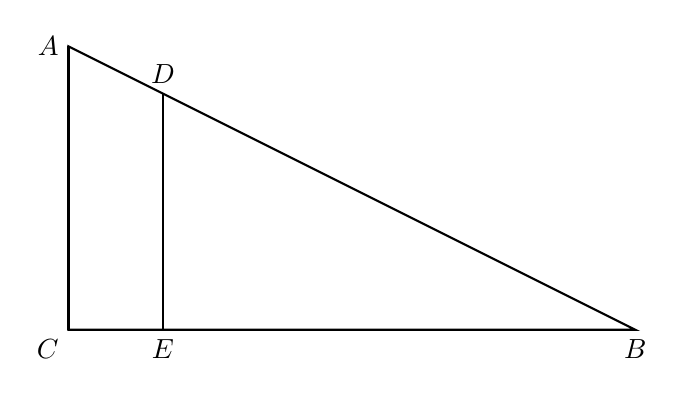
\begin{tikzpicture}[scale=0.6]
      \coordinate [label=left:$A$](A) at (-12,6);
      \coordinate [label=below:$B$](B) at (0, 0);
      \coordinate [label=below left:$C$](C) at (-12,0);
      \coordinate [label=above:$D$](D) at (-10, 5);
      \coordinate [label=below:$E$](E) at (-10,0);
      \draw [thick] (A)--(B)--(C)--cycle;
      \draw [thick] (A)--(C);
      \draw [thick] (D)--(E);
    \end{tikzpicture}
  \end{flushright}
  \item Find $AD$.
  \end{enumerate} \vspace{2.5cm}

\item As shown in the diagram, the radius of a cone is 2.5 cm and its slant height is 6.5 cm.%\\[0.5cm]
  \begin{enumerate}
    \item Find the height of the cone.
    \begin{flushright}
      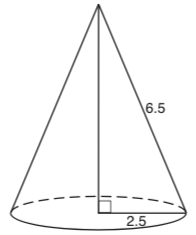
\includegraphics[width=0.25\textwidth]{cone_Jan2019-23.png}
    \end{flushright} %\vspace{2cm}
    \item How many cubic centimeters are in the volume of the cone? Express your answer in terms of $\pi$.
  \end{enumerate}

\end{enumerate}
\end{document}
